 
\chapquote{``Design is choosing how you will fail."}{Ron Fein}

\problem

\solution

\tikzstyle{vertex}=[draw]
\tikzstyle{edge}=[draw, -latex, >=stealth, line width=0.2mm]

\begin{figure}[htpb]
\begin{center}
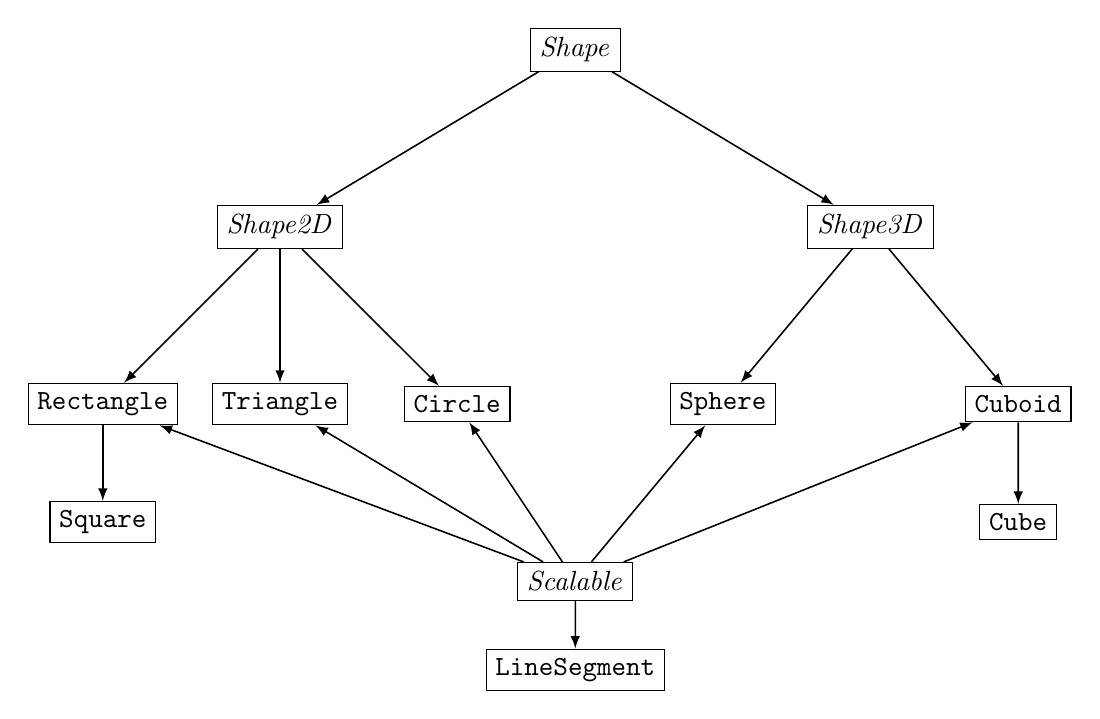
\begin{tikzpicture}[scale=0.75, auto]
	\foreach \pos/\name in {{(6,4)/Circle}, {(3,4)/Triangle}, {(0,4)/Rectangle}, {(0,2)/Square},
				{(10.5,4)/Sphere}, {(15.5,4)/Cuboid}, {(15.5,2)}/Cube, {(8,-0.5)/LineSegment}}
		\node[vertex] (\name) at \pos {\texttt{\name}};
	\foreach \pos/\name in {{(8,10)/Shape}, {(3,7)/Shape2D}, {(13,7)/Shape3D}, {(8,1)/Scalable}}
		\node[vertex] (\name) at \pos {\textit{\name}};
	\foreach \source/\dest in {Shape/Shape2D, Shape/Shape3D, Shape2D/Circle, Shape2D/Triangle,
				   Shape2D/Rectangle, Rectangle/Square, Shape3D/Sphere, Shape3D/Cuboid, Cuboid/Cube,
				   Scalable/LineSegment, Scalable/Circle, Scalable/Rectangle, Scalable/Triangle,
				   Scalable/Sphere, Scalable/Cuboid}
		\path[edge] (\source) -> (\dest);
\end{tikzpicture}
\end{center}
\label{fig:shape_tree}
\end{figure}

\algorithm

\sourcecode
\lstinputlisting{src/Scalable.java}
\lstinputlisting{src/LineSegment.java}
\lstinputlisting{src/Shape.java}
\lstinputlisting{src/Shape2D.java}
\lstinputlisting{src/Circle.java}
\lstinputlisting{src/Triangle.java}
\lstinputlisting{src/Rectangle.java}
\lstinputlisting{src/Square.java}
\lstinputlisting{src/Shape3D.java}
\lstinputlisting{src/Sphere.java}
\lstinputlisting{src/Cuboid.java}
\lstinputlisting{src/Cube.java}

\varDescription
